\documentclass[conference]{IEEEtran}

% Document properties
\title{Order-exploiting routing table minimization for a multicast supercomputer network}
\author{%
  \IEEEauthorblockN{Andrew~Mundy and Jim~D.~Garside}
  \IEEEauthorblockA{\{\texttt{andrew.mundy}, \texttt{jim.garside}\}\texttt{@manchester.ac.uk}\\
                    School of Computer Science,\\
		    University of Manchester,\\
                    M13 9PL, UK}
}

% Prettier tables
\usepackage{booktabs}

% Pictures
\usepackage{graphicx}

% Pseudo-code
\usepackage{clrscode3e}

% Force float positions in some cases
\usepackage{float}

% Neaten the fixed-width font
\usepackage{sourcecodepro}
\newcommand{\mytt}[1]{\texttt{\footnotesize#1}}

\begin{document}
  \maketitle

  \begin{abstract}
SpiNNaker is a many-core supercomputer, designed for the simulation of large neural-networks; cores communicate with multicast packets.
Routeing within SpiNNaker is controlled by ternary content addressable memories (TCAM) of quite limited size, efficient use of which allows more flexibility in the neural-networks to be simulated.
We present an algorithm for the minimization of multicast routeing tables which exploits the ordered nature of the TCAM.
This algorithm -- which fits in the small, local memory of a SpiNNaker core -- is shown to outperform the compression ratio achieved by use of Espresso on a wide sample of routeing tables.

  \end{abstract}

  \section{Introduction}

SpiNNaker [REF] is a purpose-built supercomputer intended to facilitate the simulation of large Spiking Neural Networks.
Software models are distributed across a network of processors which communicate by passing (short) messages.
Biological neurons in a brain typically have a `fanout' of the order of thousands; SpiNNaker's interconnection structure reflects this in that it supports multicasting packets to an arbitrary set of destinations.

Routeing these packets is done by Address Event Representation (AER)~[REF]; the packet source is identified and routers forward and may duplicate packets which they recognise.
SpiNNaker comprises custom silicon where each chip has a single router capable of steering packets to or from the 18 on-chip computer cores and inter-chip links.
The inter-chip network is intended to be a triangularly connected 2D surface, nominally wrapped into a torus to provide greater aggregate bandwidth.
This can be drawn as a hexagonal mesh but is sometimes more conveniently pictured skewed into squares.
The six inter-chip links are typically labelled with compass points (fig. ???).

The routeing key is a 32-bit value which reflects the intended scale of the system: $\sim2^{16}$ chips carry $\sim10^6$ processors or $\sim10^9$ neurons.
Because keying every value on every chip is impractical only selected packets are recognised on a given node.
Unrecognised packets are routed in a straight line, e.g.\ from west to east.
Packets are recognised using a Ternary Content Addressable Memory (TCAM) which will bit-mask a key before looking for particular matches.
This means that each key bit can be matched with binary \mytt{0}, \mytt{1}, or \mytt{X}, the last being a `don't care'.
The TCAM was chosen with an arbitrary size of 1024 entries, believed large enough for most applications although making entries quite precious.
It is prioritised so that only the first-found match will be returned which will generate a 24-bit output bit vector (18 local processors + 6 inter-chip links).
However, examples in this paper have been shortened for clarity.

  For example, any packets with the keys \mytt{0111} or \mytt{1111} would match the second entry in the table

  \begin{table}[H]
    \centering
    \begin{tabular}{c c l}
      \toprule
      Key & Mask & Route \\
      \midrule
      \texttt{0000} & \texttt{1111} & North East, North \\
      \texttt{0111} & \texttt{0111} & South \\
      \bottomrule
    \end{tabular}
  \end{table}

  \noindent as \mytt{0b0111 \& 0b0111 == 0b0111} and \mytt{0b1111 \& 0b0111 == 0b0111} and would thus be routed out of the South link.
  Packets with the key \mytt{0000} would instead match only the first entry and would thus be routed out of both the North East and North links.

  \subsection{Notation}

  Any bits where the key and mask of an entry are both \mytt{0} will match either \mytt{0} or \mytt{1} in packet keys and are effectively ``don't cares'' -- written as \mytt{X}.
  In addition, the routes \{East, North East, North, West, South West, South\} and Cores 0 to 17 can be shortened to \mytt{E}, \mytt{NE}, \mytt{N}, \mytt{W}, \mytt{SW}, \mytt{S} and \mytt{0} to \mytt{17} respectively.
  In this notation the above routing table is written as:

  \begin{table}[H]
    \centering
    \begin{tabular}{c l}
      \toprule
      Key-Mask & Route \\
      \midrule
      \texttt{0000} & \texttt{NE N}\\
      \texttt{X111} & \texttt{S}\\
      \bottomrule
    \end{tabular}
  \end{table}

  \subsection{Entry priority and default routing}

  In the case that a packet matches multiple routing entries only the entry nearest the top of the table has effect.
  For example, in the table

  \begin{table}[H]
    \centering
    \begin{tabular}{c l}
      \toprule
      \texttt{1100} & \texttt{E 3}\\
      \texttt{110X} & \texttt{17}\\
      \bottomrule
    \end{tabular}
  \end{table}

  \noindent any packet with the key \mytt{1100} would match both entries but only the first would have any effect (i.e., the packet would be routed out of the East link and to Core 3).
  Consequently ``catch all'' rules may be instantiated near the bottom of the table to route packets which do not match any of the entries above them.

  If a packet does not match \textit{any} entry in the routing table then it is routed out of the link opposite to the link through which it arrived at the router (e.g., out of the North link if it arrived on the South link).
  This behaviour of the router may be considered as being equivalent to there being a large number of implicit entries at the bottom of the routing table.

  \subsection{Merging routing table entries}

  Routing tables can be minimized by merging together entries with equivalent routes.
  This is done by creating a new key-mask pair with an \mytt{X} in any bit wherever the key-mask pairs of any of the original entries differed or already contained an \mytt{X}.
  For example, merging the entries:

  \begin{table}[H]
    \centering
    \begin{tabular}{c l}
      \toprule
      \texttt{0000} & \texttt{N}\\
      \texttt{0001} & \texttt{N}\\
      \bottomrule
    \end{tabular}
  \end{table}

  \noindent would result in the new entry:

  \begin{table}[H]
    \centering
    \begin{tabular}{c l}
      \toprule
      \texttt{000X} & \texttt{N}\\
      \bottomrule
    \end{tabular}
  \end{table}

  \noindent which matches exactly the keys matched by the original entries.
  In contrast, merging the entries \mytt{0001} and \mytt{0010} would result in \mytt{00XX} which would match any packets with the keys \mytt{0000} and \mytt{0011} \textit{in addition} to those matched by the original entries.

  Clearly, care must be taken if tables such as

  \begin{table}[H]
    \centering
    \begin{tabular}{c l}
      \toprule
      \texttt{0001} & \texttt{N}\\
      \texttt{0010} & \texttt{N}\\
      \texttt{0000} & \texttt{SW S}\\
      \texttt{0011} & \texttt{SW}\\
      \bottomrule
    \end{tabular}
  \end{table}

  \noindent are to remain functionally equivalent after minimization -- as, for example, merging the first two entries and leaving the result in place would result in the functionally different:

  \begin{table}[H]
    \centering
    \begin{tabular}{c l}
      \toprule
      \texttt{00XX} & \texttt{N}\\
      \texttt{0000} & \texttt{SW S}\\
      \texttt{0011} & \texttt{SW}\\
      \bottomrule
    \end{tabular}
  \end{table}

  \subsection{Orthogonality}

  A routing table is orthogonal if are no keys that are matched by multiple table entries.
  For example, the following tables are functionally equivalent but the left-hand table is non-orthogonal as the key \mytt{1110} is matched by both entries in the table:

  \begin{figure}[H]
    \centering
    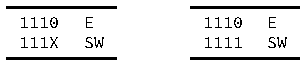
\includegraphics{figures/orthogonality}
  \end{figure}

  It is typically easier to minimize orthogonal routing tables, but it should be noted that minimizing a table will often (but not always) produce a non-orthogonal table.
  Consequently any algorithm which proceeds by repeatedly applying minimization steps to a table must be capable of working with non-orthogonal tables; for this reason some of the examples in this paper use non-orthogonal tables.

  \section{Order-exploiting routing table minimization}

  The algorithm presented in this paper provides two rules which guide how routing tables may be minimized through merging of entries:

  \begin{enumerate}[\IEEEsetlabelwidth{2)}]
    \item Routing tables are to be kept sorted in increasing order of the number of \mytt{X}s contained in their keys and masks, that is in increasing order of \textit{generality}.
      For example, an entry with the key-mask of \mytt{00XX} (\textit{generality} of 2) must be placed below any entries with fewer \mytt{X}s in their key-masks, e.g., below \mytt{0000} and \mytt{00X1} (generalities of 0 and 1 respectively).
      \begin{enumerate}[\IEEEsetlabelwidth{a)}]
        \item Additionally, new entries must be inserted below existing entries of equivalent generality.
              For example, if \mytt{XX00} were already present in the table the new entry \mytt{0XX1} must be inserted below it.
      \end{enumerate}
    \item Any merge may be made provided that it would not
      \begin{enumerate}[\IEEEsetlabelwidth{b)}]
        \item cause any entry in the merge to become \textit{covered} by an entry higher up the table.
              A merge that would be disallowed by this rule is shown in \figurename~\ref{fig:algorithm/rule2a_example}.
              This rule is referred to as the \textit{up-check} rule.
        \item cause any entry below the merge to become covered (see \figurename~\ref{fig:algorithm/rule2b_example}).
              This rule is referred to as the \textit{down-check} rule.
      \end{enumerate}
  \end{enumerate}

  \begin{figure}
    \centering
    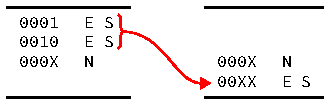
\includegraphics{figures/rule2a_example}
    \caption{
      Example of a merge which does not obey rule~(2a), the \textit{up-check}.
      Before the merge a packet with key \mytt{0001} would have been routed to \mytt{E~S}; after the merge the same packet would be routed to \mytt{N} instead.
      This is because the merge has resulted in the correct entry being moved below an entry which \textit{covers} it.
    }
    \label{fig:algorithm/rule2a_example}
  \end{figure}

  \begin{figure}
    \centering
    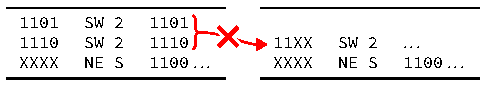
\includegraphics{figures/rule2b_example}
    \caption{
      Example of a merge which does not obey rule~(2b), the \textit{down-check}.
      Before the merge a packet with key \mytt{1100} would have been routed to \mytt{NE~S}; after the merge the same packet would be routed to \mytt{SW 2} instead.
      This is because the merge has resulted in the insertion of a new entry which \textit{covers} an existing entry.
    }
    \label{fig:algorithm/rule2b_example}
  \end{figure}

  These rules may be transformed into a simple, greedy, algorithm to minimize a routing table:

  \begin{codebox}
    \Procname{$\proc{Minimize}(\id{table}, \id{target})$}
    \li \While $\attrib{table}{length} >  \id{target}$
    \li \Do $\id{merge} \gets \proc{Get-Largest-Merge}(\id{table})$
    \li     \If $\attrib{merge}{isEmpty}$
    \li     \Then \kw{break} \End
    \li     $\id{table} \gets \proc{Apply-Merge}(\id{table}, \id{merge})$
        \End
    \li \Return $\id{table}$
  \end{codebox}

  \noindent Where:
  \begin{itemize}
    \item $\id{table}$ is a routing table that is sorted according to rule~(1)
    \item $\proc{Get-Largest-Merge}$ is a function which returns a (possibly empty) set of routing table entries which may be merged without breaking rule~(2)
    \item $\proc{Apply-Merge}$ applies a merge to a routing table using rule~(1) to determine where the new entry should be inserted
  \end{itemize}

  Initially $\proc{Get-Largest-Merge}$ should immediately reject any merge which breaks either rule~(2a)~or~(2b).
  However, this will lead to very poor minimization.
  To improve performance methods are required which modify potential merges to obey both rules.

  \subsection{Resolving the up-check}

  Consider the table

  \begin{figure}[H]
    \centering
    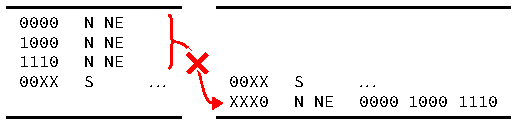
\includegraphics{figures/upcheck_resolve_example_1}
  \end{figure}

  \noindent Initially we consider merging the first three entries.
  Doing so, however, would involve moving the first matching entry for \mytt{0000} below \mytt{0X00} which would break rule~(2a).
  To resolve this we can remove \mytt{0000} from the merge, resulting in:

  \begin{figure}[H]
    \centering
    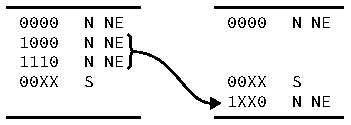
\includegraphics{figures/upcheck_resolve_example_2}
  \end{figure}

  \textbf{TODO: Express this algorithmically, explain the effects}

  \subsection{Resolving the down-check}
  
  Rule~(2b) disallows any merges which would create a new entry that would cover any entries below the point where it would be inserted.
  However, if routing table entries are annotated with the keys (expressed as key-masks) that they are expected to match then rule~(2b) can be re-expressed as:

  \begin{quote}
    Any merge may be made provided that it would not cause any key which is expected to be matched by an entry below the merge to become covered.
  \end{quote}

  \figurename~\ref{fig:algorithm/rule2b'_example} shows an example of a merge which would previously have been disallowed by rule~(2b) but would be valid given extra information and this revision to rule~(2b).

  \begin{figure}
    \centering
    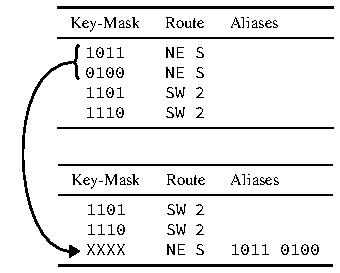
\includegraphics{figures/aliases_example}
    \caption{
      Example of a merge which does not obey rule~(2b), the \textit{down-check}, but is valid if extra information about which keys are expected to reach which entries is provided.
      While the merge would result in a packet with key \mytt{1100} being routed differently, \textit{no such packet is expected to reach the bottom routing table entry} and neither of the keys that are expected (\mytt{1011} and \mytt{0100}) will match the entry inserted by the merge (\mytt{11XX}).
    }
    \label{fig:algorithm/rule2b'_example}
  \end{figure}

  Consider the table:

  \begin{table}[H]
    \centering
    \begin{tabular}{c l l}
      \toprule
      Key-Mask & Route & Aliases \\
      \midrule
      \texttt{1100} & \texttt{N} \\
      \texttt{1101} & \texttt{N} \\
      \texttt{111X} & \texttt{N} \\
      \texttt{XXXX} & \texttt{4} & \texttt{0100}, \texttt{1011}, \texttt{1110} \\
      \bottomrule
    \end{tabular}
  \end{table}

  The first three entries cannot be merged because the merged entry (\mytt{11XX}) would be inserted above the bottom entry and would prevent packets with the key \mytt{1110} from being routed correctly.

  To proceed we attempt to find bits which are \mytt{X}s in the merged entry but are not \mytt{X}s in the covered entry.
  In this example this is the two rightmost bits, \mytt{11\underline{XX}} and \mytt{11\underline{10}} for the merged and covered entries respectively.
  To resolve the covering we attempt to remove entries from the merge such that one of the \mytt{X}s we just identified becomes the opposite of the covered value in the same position.
  In this example, we look to remove entries from the merge such that the merged entry is either \mytt{11\underline{X1}} or \mytt{11\underline{0X}}.

  \textbf{TODO: Finish this example, express algorithmically, explain the effects.}

  \subsection{The complete algorithm}

  \section{Results}

  \subsection{Compression ratio}

  \subsection{On-chip performance}

  \section{Discussion}

  \section{Conclusion}
\end{document}
